\section{Methodology}
\label{sec:method}

We develop \ours as an open framework for composing world prediction and
action generation. It combines three ingredients: a causal video backbone
pretrained on robot video without action labels, a common video--action
architecture whose cross-modal interaction can be reconfigured, and
separately trained inverse and forward dynamics components operating through
local trajectory interfaces.

The design supports two forms of composition. At the \emph{architectural}
level, we vary how future observation and action streams interact while
retaining a common backbone and objective family. At the
\emph{component} level, we connect independently trained predictors through
explicit future-observation and action-trajectory interfaces. The latter
motivates local-context dynamics models that do not require the language and
nonlocal history used by a task-conditioned generator.


% \subsection{Composable World--Action Modeling}
\subsection{World--Action Modeling Formulation}
\label{sec:world-action-interfaces}

Let \(o_t \in \mathcal{O}\), \(a_t \in \mathcal{A}\), \(q_t \in \mathcal{Q}\), and \(\ell\in\mathcal{L}\) denote the visual observation, action, proprioceptive state, and language instruction at time $t$. For fixed observation- and action-history lengths \(K_o\in\mathbb{N}\) and \(K_a\in\mathbb{N}\), respectively, we define
\begin{equation}
\begin{aligned}
O_t^- &= (o_{t-K_o}, \ldots, o_{t-1}), \\
A_t^- &= (a_{t-K_a}, \ldots, a_{t-1}), \\
O_t^0 &= o_t.
\end{aligned}
\end{equation}

Let \(H\in\mathbb N_{>0}\) denote the prediction horizon. The future action and observation trajectories are defined as
\begin{equation}
% \begin{aligned}
A_t^+ = (a_t, \ldots, a_{t+H-1}), \quad O_t^+ = (o_{t+1}, \ldots, o_{t+H}).
% \end{aligned}
\end{equation}

We collect the information available before predicting the future into the task context
\[
\mathcal C_t=(O_t^-,O_t^0,A_t^-,q_t,\ell).
\]

Recorded future trajectories are denoted without hats, whereas generated trajectories are denoted by \(\hat O_t^+\) and \(\hat A_t^+\). We omit the time index \(t\) when it is unambiguous.

\ours models future observations and actions jointly. For a reference
joint distribution, the two chain-rule factorizations are
\begin{equation}
\begin{aligned}
p_{\mathrm{WAM}}
( O_t^+, A_t^+\mid\mathcal C_t)
&=
\underbrace{p( O_t^+\mid\mathcal C_t)}_{\mathrm{CVP}}
\underbrace{
p( A_t^+\mid O_t^+,\mathcal C_t)
}_{\mathrm{IDM}}\\
&=
\underbrace{p( A_t^+\mid\mathcal C_t)}_{\mathrm{VLA}}
\underbrace{
p( O_t^+\mid A_t^+,\mathcal C_t)
}_{\mathrm{FDM}}.
\end{aligned}
\label{eq:wam-factorizations}
\end{equation}
Causal video prediction (CVP) proposes future observations, a direct
vision--language--action (VLA) policy proposes actions, inverse dynamics
(IDM) grounds a supplied visual transition into actions, and forward
dynamics (FDM) predicts the visual consequence of supplied actions.

These roles give three primary generation routes.
\emph{Joint generation} produces future observations and actions
concurrently. \emph{Video-then-action (VTA)} first generates a visual
future and then conditions action generation on that trajectory.
\emph{Action-then-video (ATV)} first proposes actions and then predicts
their visual consequences. These factorizations specify modeling
interfaces; they do not require all factors to share one trained
parameterization or final checkpoint.




\subsection{An Open Causal Robot-Video Backbone}
\label{sec:causal-video-backbone}

% We initialize the visual backbone from Wan2.2-5B~\cite{wan2025wan} and
% further pretrain it on heterogeneous robot and interaction video without action labels. This stage
% adapts a general video prior toward robot-centric motion and interaction
% while retaining a standalone predictive model. The resulting checkpoint
% provides the common visual initialization for the downstream world--action
% configurations. Dataset composition and optimization settings are given in
% Sec.~\ref{sec:experimental-setup}. We release the robot-video-pretrained
% checkpoint and its training recipe for standalone prediction and downstream
% world--action modeling.

We initialize the video backbone from Wan2.2-5B~\cite{wan2025wan} and
continue pretraining it on heterogeneous robot-manipulation and interaction
videos without action supervision. This stage adapts a general-purpose video
prior to robot-centric motion and interaction while preserving a standalone
video-prediction interface. The resulting checkpoint is shared across all
downstream \ours variants, allowing different video--action interaction
strategies to be compared under a common visual initialization. Dataset
composition and optimization details are summarized in
Sec.~\ref{sec:experimental-setup}.

Because the original video model is not temporally causal, we introduce
chunk-causal prediction during robot-video pretraining. A future chunk may
attend to the current and preceding observations and previously generated
chunks, but not to later chunks; tokens within a chunk are processed
jointly. This provides the temporal direction needed for sequential
prediction while retaining within-chunk denoising.

Temporal causality and cross-modal interaction are separate design
dimensions. Chunk causality determines which times are visible, while the
interaction programs in Sec.~\ref{sec:interaction-programs} determine which
observation and action streams communicate. The pretrained causal backbone
can therefore be used directly as a video predictor or coupled to an action
branch without changing its basic predictive interface.


\subsection{Configurable Video--Action Interaction Programs}
\label{sec:interaction-programs}
\label{sec:framework-architecture}

\paragraph{Shared architecture.}
We couple the pretrained video backbone to a separate action
transformer using a Mixture-of-Transformers (MoT) architecture \cite{liang2024mixture}. Video and
action trajectories are encoded into temporally aligned streams and
processed by modality-specific transformer branches. Interleaved
cross-modal attention determines how information flows between them. The
backbone, tokenization, and objective family are shared across
configurations; future cross-modal visibility and generation order are the
principal variables. Figure~\ref{fig:openwam-mot-programs} summarizes the
architecture, and Figure~\ref{fig:openwam-masks} the attention masks of four
interaction programs together with the two local-context dynamics programs.

\begin{figure}[t]
  \centering
  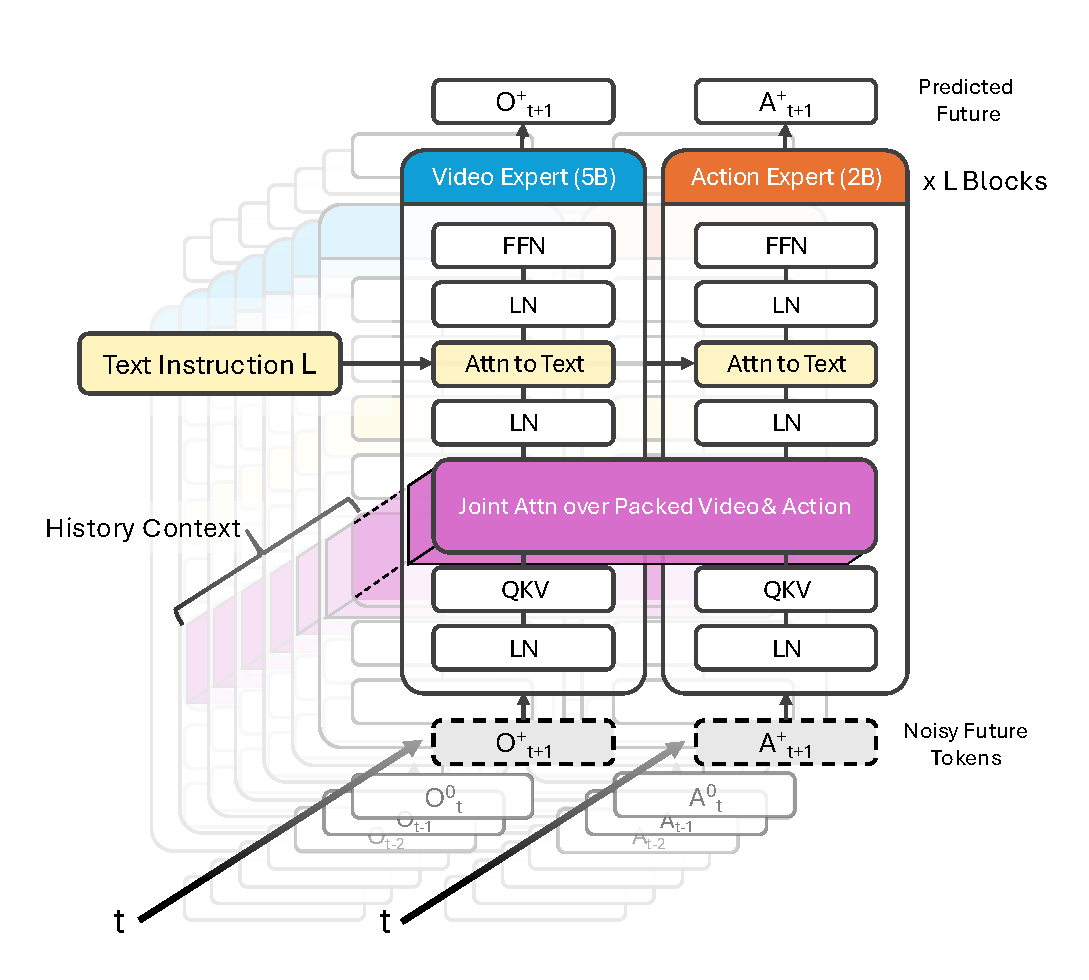
\includegraphics[width=\linewidth]{sec/images/openwam-fig2-arch-v1.pdf}
  % \vspace{-0.4in}
  \caption{
  Shared MoT architecture. Two modality-specific branches keep their own
  normalization, projection and feed-forward parameters and meet in a single
  attention over the packed video and action tokens; a separate
  cross-attention consumes the task text. Noisy future tokens enter at the
  bottom and the preceding chunks sit behind as history context.
  }
  \label{fig:openwam-mot-programs}
\end{figure}


\paragraph{Interaction programs.}
We study four video--action interaction programs under a shared
Mixture-of-Transformers backbone. \emph{Joint} denoises future video and
action streams concurrently, with bidirectional attention between their
noisy future tokens. \emph{VTA} first predicts future video without access
to future actions, then predicts the action conditioned on the
completed visual trajectory. \emph{ATV} reverses this order: it first
predicts the action, then conditions video prediction on the
completed action trajectory. \emph{Decoupled} predicts both modalities
without future cross-modal attention. All four programs use the same backbone, tokenization, and
training objective; they differ only in generation order and future
cross-modal attention.



\begin{figure}[t]
  \centering
  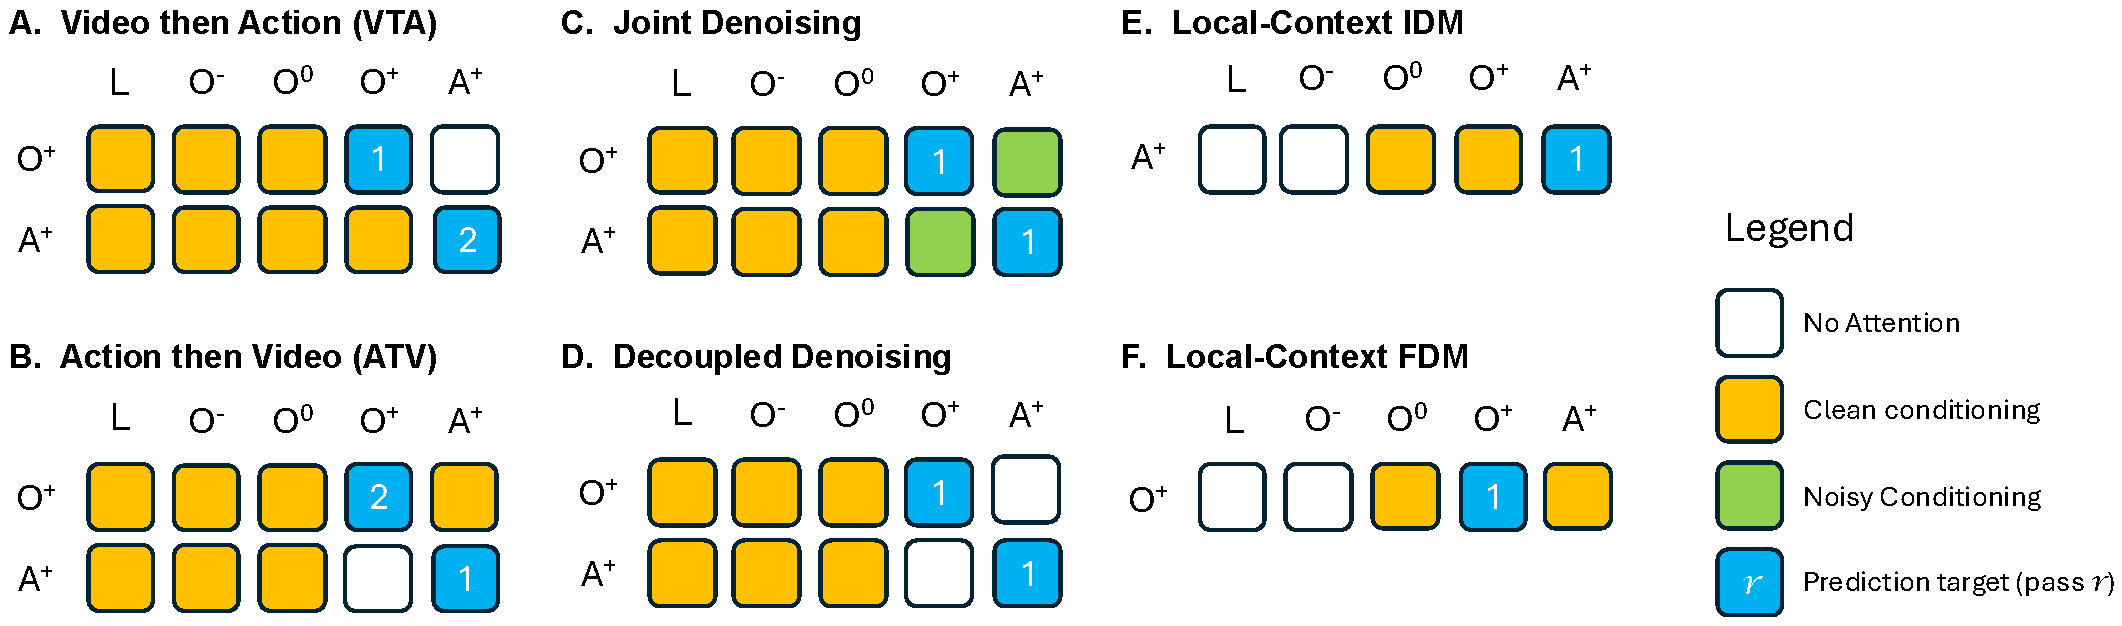
\includegraphics[width=0.98\linewidth]{sec/images/openwam-fig3-masks-v1.pdf}
    % \vspace{-0.1in}
  \caption{
  Attention masks the shared architecture exposes: four interaction programs
  (A--D) and the two local-context dynamics programs (E--F). Columns are the
  streams a row may condition on, cell colour gives what it attends to there,
  and the numeral marks the generation pass. E and F carry one row each
  because each predicts a single stream: the inverse model produces actions, the forward model observations.
  }
  \label{fig:openwam-masks}
  % \vspace{-0.1in}
\end{figure}


\begin{table}[t]
    \centering
    \caption{LIBERO-90 targets used for component-transfer evaluation.}
    % \vspace{-0.1in}
    \label{tab:transfer-tasks}
    \small
    \resizebox{\linewidth}{!}{%
    \begin{tabular}{@{}cll@{}}
        \toprule
        \textbf{Task}
        & \textbf{Target behavior}
        & \textbf{Transfer challenge} \\
        \midrule
        64
        & Stack bowls; place stack in tray
        & Novel skill composition \\
        74
        & Book into caddy's left compartment
        & Retarget familiar manipulation \\
        21
        & Turn on stove; place frying pan on it
        & Object and grasp change \\
        45
        & Same objective as Task 21
        & Additional scene and layout shift \\
        \bottomrule
    \end{tabular}}
    % \vspace{-0.2in}
\end{table}

\begin{figure*}[t]
  \centering
  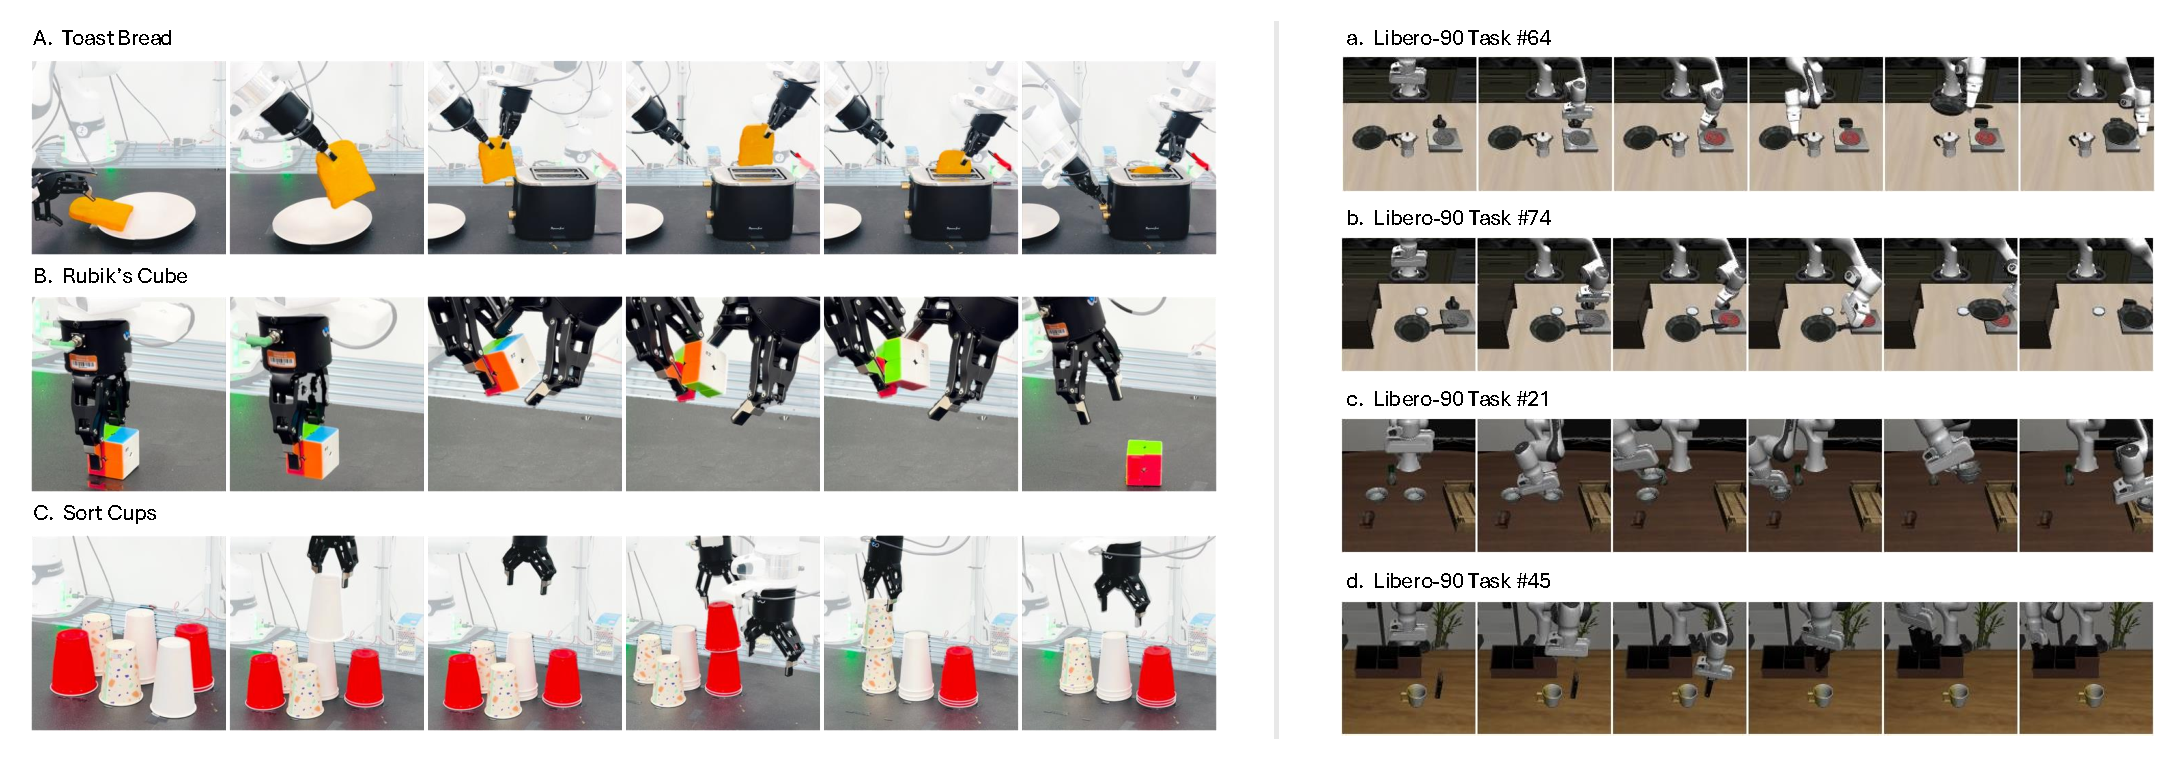
\includegraphics[width=0.98\linewidth]{sec/images/openwam-fig3-tasks-v1.pdf}
  % \vspace{-0.2in}
  \caption{Evaluation tasks. \textbf{Left:} the three real-world bimanual
  tasks of Table~\ref{tab:real-world-tasks}, each shown as frames sampled
  along one successful rollout. \textbf{Right:} the four LIBERO-90 targets of Table~\ref{tab:transfer-tasks} used for component transfer, which lie
  outside the LIBERO-Long source-task set.}
  \label{fig:tasks}
  % \vspace{-0.1in}
\end{figure*}

\paragraph{Shared flow-matching objective.}
All programs use the same latent flow-matching~\cite{lipman2022flow} construction. For target
modality $P\in\{\mathrm O,\mathrm A\}$, let $Z_P^\star$ be its clean target
latent. With $\tau\sim\mathcal U[0,1]$ and
$\epsilon_P\sim\mathcal N(0,I)$,
% \begin{equation}
% \begin{aligned}
% Z_{P,\tau}&=(1-\tau)\epsilon_P+\tau Z_P^\star,\\
% u_P&=Z_P^\star-\epsilon_P.
% \end{aligned}
% \label{eq:flow-path}
% \end{equation}
\begin{equation}
Z_{P,\tau}=(1-\tau)\epsilon_P+\tau Z_P^\star,\quad
u_P=Z_P^\star-\epsilon_P.
\label{eq:flow-path}
\end{equation}
An active prediction stage minimizes
\begin{equation}
\mathcal L_P
=
\mathbb E\!\left[
\left\|
v_{\theta,P}
\!\left(
Z_{P,\tau}\mid c_P,\tau
\right)
-u_P
\right\|_2^2
\right],
\label{eq:shared-flow-objective}
\end{equation}
where $c_P$ denotes the history, side information, and cross-modal
trajectory made visible by the interaction program. Programs with
multiple targets sum the corresponding losses. Observation and
action trajectories used as conditioning are processed through their
respective modality encoders.

% During training, the second stage of a sequential program conditions on the
% recorded cross-modal trajectory rather than a sampled first-stage output;
% this conditioning may be stochastically corrupted according to the training
% configuration. At inference, it is replaced by the completed trajectory
% generated by the first stage. The complete token-level visibility masks,
% corruption schedules, temporal alignment, chunk configuration, and sampling
% procedure are provided in the appendix.
During training, a sequential program uses teacher forcing: the second
generation pass conditions on the recorded cross-modal trajectory rather than
on an output sampled by the first pass. At inference, it conditions on the
completed trajectory generated by the first pass. The same interaction program
and temporal alignment are used during training and inference; the source of the conditioning trajectory changes
from recorded to generated. 
% The history-stream visibility settings of the
% examined checkpoints and evaluation launcher are documented in
% Sec.~\ref{sec:supp-compute}.



\subsection{Counterfactual Learning of Local-Context Dynamics Interfaces}
\label{sec:strict-dynamics}

\paragraph{Local-context dynamics interfaces.}
Architectural composition controls communication within a model, but
reusing a separately trained component requires an explicit conditioning
boundary. A task-conditioned generator may use language and nonlocal
history to specify behavior; a reusable local dynamics component instead
relates a supplied transition to its actions, or supplied actions to their
consequences.

We therefore define
\begin{equation}
\begin{aligned}
p_{\mathrm{IDM}}^{\mathrm{local}}
&:=
p(
 A_t^+
\mid
 O_t^+, O_t^0,q_t
),\\
p_{\mathrm{FDM}}^{\mathrm{local}}
&:=
p(
 O_t^+
\mid
 A_t^+, O_t^0,q_t
).
\end{aligned}
\label{eq:strict-modeling-roles}
\end{equation}
% \begin{equation}
% p_{\mathrm{IDM}}^{\mathrm{local}} := p(A_t^+ \mid O_t^+, O_t^0, q_t),
% \qquad
% p_{\mathrm{FDM}}^{\mathrm{local}} := p(O_t^+ \mid A_t^+, O_t^0, q_t).
% \label{eq:strict-modeling-roles}
% \end{equation}
Local-context IDM grounds a supplied visual trajectory into an action sequence,
while local-context FDM predicts the visual consequence of a supplied action
sequence. Neither receives language, past actions, or observations
preceding $t$.

Importantly, conditioning scope and transition supervision are separate
design choices. The local-context restriction specifies which variables the dynamics component
may consume; it does not determine which transitions are used for learning.
Conversely, broader transition supervision can also be applied to a
full-context dynamics model. Sec.~\ref{sec:component-composability}
therefore compares full-context and local-context IDMs under matched
demonstration-only and mixed supervision.

% Local-context conditioning is an input restriction, not an assumption that the
% current observation is universally sufficient to determine local dynamics.
% Formal local-sufficiency conditions and their qualifications are provided
% in the appendix; we evaluate the adequacy of the restricted interface
% empirically through local prediction and composed control.
Local-context conditioning restricts the variables available to the dynamics
component; it does not assume universal local sufficiency. Its adequacy
depends on whether the information needed for local action--outcome inference
is observable from the current observation, proprioceptive state, and supplied
transition. We evaluate this interface through local prediction and composed
control.

\paragraph{Broader local-transition supervision.}
A task trajectory induces a local transition
$z=( O_t^0,q_t, A_t^+, O_t^+)$.
Let $\mathcal D_{\mathrm{task}}^{\mathrm{loc}}$ denote the distribution of
such transitions obtained from demonstrations. Demonstrations provide valid
transitions but contain only the action continuations selected by the
policy.

To broaden local supervision, we restore selected simulator states and
execute alternative future action sequences. For branch $b$, this produces
$z^{(b)}=( O_t^0,q_t, A_t^{+,(b)},
 O_t^{+,(b)})$, where the initial condition is shared and each
future observation trajectory results from executing its corresponding
action sequence. These alternatives include interactions outside the
demonstrated continuation and need not complete the task. The simulator
state is used only to control data collection and is not provided to the
model.

The paired collection protocol controls the starting state, while the
learning objective operates on individual transition records rather than
using an explicit paired-branch loss. Let $\mathcal D_{\mathrm{cf}}$ denote
the resulting counterfactual transitions. Dynamics models are trained from
\begin{equation}
\mathcal D_{\mathrm{dyn}}
=
(1-\eta)\mathcal D_{\mathrm{task}}^{\mathrm{loc}}
+
\eta\mathcal D_{\mathrm{cf}},
\qquad
\eta\in[0,1].
\label{eq:dynamics-training-distribution}
\end{equation}
This supports demonstration-only, counterfactual-only, and mixed
supervision without changing the conditioning interface. The experimental
mixture and collection details are given in Sec.~\ref{sec:experimental-setup}.
% The same local-transition representation also accommodates naturally occurring failed attempts and play in the physical-robot setting.
The same interface can be applied to failed or exploratory physical-robot transitions when such data are collected.

\paragraph{Local dynamics learning.}
Using the flow construction in Eq.~\ref{eq:flow-path}, local-context IDM denoises
the action target while conditioning on the observed future, whereas local-context
FDM denoises the future observation target while conditioning on the
executed action sequence:
\begin{equation}
\begin{aligned}
\mathcal L_{\mathrm{LC\text{-}IDM}}
&=
\mathbb E\!\left[
\left\|
v_{\theta_{\mathrm{ID}}}
(
Z_{\mathrm A,\tau}
\mid
 O^0,q_t, O^+,\tau
)
-u_{\mathrm A}
\right\|_2^2
\right],\\
\mathcal L_{\mathrm{LC\text{-}FDM}}
&=
\mathbb E\!\left[
\left\|
v_{\theta_{\mathrm{FD}}}
(
Z_{\mathrm O,\tau}
\mid
 O^0,q_t, A^+,\tau
)
-u_{\mathrm O}
\right\|_2^2
\right].
\end{aligned}
\label{eq:strict-dynamics-objectives}
\end{equation}
Ground-truth future observations condition IDM training but are not video
denoising targets; analogously, executed actions condition FDM training.


\paragraph{Inference and component composition.}


For video-to-action composition, the video predictor passes future
variational autoencoder (VAE) video latents to the receiving IDM;
transformer hidden states and caches are not transferred across components.
The receiving IDM processes the transferred latents through the same
modality-conditioning pathway used for recorded conditioning.
% Detailed tensor layouts and encoding configuration are given in the appendix.

At inference, a task-conditioned visual predictor can be paired with an
independently trained local-context IDM:
% \begin{equation}
% \begin{aligned}
% \hat{ O}_t^+
% &\sim
% p_\phi^{\mathrm{CVP}}
% (\cdot\mid\mathcal C_t),\\
% \hat{ A}_t^+
% &\sim
% p_{\theta_{\mathrm{ID}}}^{\mathrm{LC\text{-}IDM}}
% (
% \cdot
% \mid
% \hat{ O}_t^+, O_t^0,q_t
% ).
% \end{aligned}
% \label{eq:strict-vta-composition}
% \end{equation}
\begin{equation}
\hat{O}_t^+ \sim p_\phi^{\mathrm{CVP}}(\cdot\mid\mathcal C_t),
\quad
\hat{A}_t^+ \sim p_{\theta_{\mathrm{ID}}}^{\mathrm{LC\text{-}IDM}}
(\cdot\mid \hat{O}_t^+, O_t^0, q_t).
\label{eq:strict-vta-composition}
\end{equation}
Task context determines the desired future through the visual predictor,
while the receiving IDM receives only the generated future trajectory and the
current local inputs.
% Detailed temporal masking is given in the appendix.

The complementary composition pairs an action generator with local-context FDM:
% \begin{equation}
% \begin{aligned}
% \hat{ A}_t^+
% &\sim
% p_\psi^{\mathrm{VLA}}
% (\cdot\mid\mathcal C_t),\\
% \hat{ O}_t^+
% &\sim
% p_{\theta_{\mathrm{FD}}}^{\mathrm{LC\text{-}FDM}}
% (
% \cdot
% \mid
% \hat{ A}_t^+, O_t^0,q_t
% ).
% \end{aligned}
% \label{eq:strict-atv-composition}
% \end{equation}
\begin{equation}
\hat{A}_t^+ \sim p_\psi^{\mathrm{VLA}}(\cdot\mid\mathcal C_t),
\quad
\hat{O}_t^+ \sim p_{\theta_{\mathrm{FD}}}^{\mathrm{LC\text{-}FDM}}
(\cdot\mid \hat{A}_t^+, O_t^0, q_t).
\label{eq:strict-atv-composition}
\end{equation}

The action sequence may equivalently be supplied by an external policy.
These are learned compositions: separately trained components need not
recover factors of one identical learned joint distribution. Their common
trajectory interfaces instead make the components explicitly replaceable,
and Sec.~\ref{sec:component-composability} evaluates when such replacement
succeeds.
